\documentclass[12pt,times,a4paper]{report}
\setlength{\textwidth}{6.25in}
\setlength{\textheight}{9in}
\renewcommand{\baselinestretch}{1.5}
\oddsidemargin 20pt
\evensidemargin 20pt
\topmargin 0.0pt
\usepackage{hyperref}
\usepackage{fancyhdr}
\usepackage{fancybox}
\usepackage[export]{adjustbox}
\usepackage{times}
\usepackage{cite}
\usepackage{graphicx}
\usepackage[left=1.25in,right=1in,top=1in,bottom=1in]{geometry}
\usepackage{hyperref}
\usepackage{amsfonts}
\usepackage{amssymb}
\usepackage{amsmath}
\usepackage{float}
\usepackage{enumitem}
\usepackage{pdfpages}
\usepackage{algorithmic}
\usepackage{algorithm}
\usepackage{comment}
\usepackage{multirow}
\usepackage{titlesec}
\usepackage{lipsum}
\usepackage{graphics}
\usepackage{graphicx}
\usepackage{fancyhdr}
\usepackage{bm,nicefrac}
\titleformat{\chapter}[display]{\Large\bfseries}%
    {\chaptername~\thechapter}{1ex}{}[\titlerule]

% Redefine the plain page style
\pagenumbering{gobble}
 \fancypagestyle{plain}
 
%certificate 
\begin{document}
\begin{titlepage}
\newpage
\addtocontents{toc}{\protect\thispagestyle{empty}}
\pagenumbering{gobble}
\pagestyle{empty}
\pagenumbering{roman}

\thispagestyle{empty}
\thisfancypage{%
  \setlength{\fboxrule}{2pt}\doublebox}{}

\begin{center}
\vspace*{0.2in}
{\fontsize{18}{16} \bf {A}}\\
{\fontsize{18}{16} \bf {Project Based Seminar Report}}\\
{\fontsize{18}{16} \it {On }}\\
\vspace*{0.2in}
{\fontsize{18}{14} \bf {\lq\lq  Prediction of values using Artificial Neural Networks \rq\rq}}\\
\vspace*{0.2in}
{\fontsize{12}{16} \bf  Submitted to the}\\
{\fontsize{12}{16} \bf Savitribai Phule Pune University
}
\begin{normalsize}
\begin{center}
In partial fulfillment for the award of the Degree of
\end{center}
\end{normalsize}

{\fontsize{14}{12} \bf  Bachelor of Engineering }\\
{\fontsize{14}{12} \bf  In}
\\{\fontsize{14}{12} \bf  Information Technology }\\
{\fontsize{12}{16} \bf   By}\\
\vspace*{0.1in}
{\fontsize{14}{12} \bf Shubham Derhgawen }\\
{\fontsize{12}{8} \bf [Exam seat No T150608505] }\\

\vspace*{0.2in}
{\fontsize{12}{16} \bf Under the Guidance of }\\
\vspace*{0.1in}
{\fontsize{14}{12} \bf Prof. Pooja Kadam}\\
\begin{figure}[h]
\centerline{
\includegraphics[scale=0.8]{logo1.jpg}}
\end{figure}

{ \fontsize{14}{12}  {Department Of Information Technology}}\\
{ \fontsize{14}{12} \bf {Dhole Patil  College Of Engineering}}\\
{ \fontsize{14}{12}  {DHOLE PATIL COLLEGE ENGINEERING, PUNE-412207 (India)}}\\

Academic year 2018-19

\end{center}
\end{titlepage}
%-------------------Cover page ends
%-------------------Certificate Starts


\begin{titlepage}
\begin{center} 
\addcontentsline{toc}{chapter}{\numberline{}Certificate}
\begin{figure}[h]

\centerline{
\includegraphics[scale=0.8]{logo1}}

\end{figure}


\vspace*{0.1in}
{\fontsize{16}{12}\textbf{{CERTIFICATE}} }\\
\begin{enumerate}
\vspace{0.3in}
This is to certify that the project based seminar report entitled \lq\lq \textbf{ Prediction of values using Artificial Neural Networks}
 \rq\rq
being submitted by \textbf{ Shubham Derhgawen (T150608505)}  is a record of bonafide work carried out by him
/her under the supervision and guidance\textbf{ Prof. Pooja Kadam } in partial fulfillment of the
requirement for \textbf{ TE (Information Technology Engineering) – 2015} course of Savitribai Phule
Pune University, Pune in the academic year 2018-2019

\vspace*{0.3in}
Date  : .........................  \\ 
Place : .........................  \\ 
 
\vspace{0.8in}
\begin{table} [h]
\addtolength{\tabcolsep}{65pt}
\begin{tabular}{c                c  }
Seminar Guide  & H.O.D \\
 Prof. Pooja Kadam  & Prof. Rahul Ghode 
\end{tabular}
\end{table}
\vspace{0.8in}
\hrulefill

This project-based seminar report has been examined by us as per the Savirtibai Phule Pune
University, Pune, requirements at Dhole Patil College of Engineering on . . . . . . . . . . . . .
\vspace{0.6in}
\begin{table} [h]
\addtolength{\tabcolsep}{65pt}
\begin{tabular}{c                c  }
Name \& Sign  & Name \& Sign \\
 Internal Examiner   & External Examiner 
\end{tabular}
\end{table}
\end{enumerate}
\end{center}

\end{titlepage}
%-------------------Certificate Ends
%-------------------Acknowledgement Starts
%\begin{titlepage}
\newpage
\begin{center}
\pagenumbering{roman}
\thispagestyle{empty}
\renewcommand{\baselinestretch}{1.5}
\addcontentsline{toc}{chapter}{\numberline{}Acknowledgement}
{\fontsize{12}{10} \bf ACKNOWLEDGEMENT}\\
%\section{ACKNOWLEDGMENT}
\begin{enumerate}
\vspace{0.4in}
The completion of report on \textbf{“Prediction of values using Artificial Neural Networks”} has given me immense pleasure and knowledge. I am sincerely thankful to Principal \textbf{Dr. N. Walimbe , Prof.Rahul Ghode} our head of the IT Department, project based seminar guide \textbf{Prof. Pooja Kadam } and project based seminar in charge \textbf{Prof. Rahul Ghode} who have cooperated with me at different stages during the preparation of this report.

My sincere thanks to the staff of Information Technologies Department without whose help it
would not have been possible for me to complete this report. This work is virtually the result of
inspiration given by them.

I would also like to thank all the library and non teaching staff for their help and last but not
least, I would like to thank all my friend for their constant help and support.

\end{enumerate}
\end{center}
\vspace*{0.8in}
{\bf Shubham Derhgawen}\\

%\end{titlepage}
%-------------------Acknowledgement Ends

%-------------------List of publication Starts
%\begin{titlepage}
\newpage

%-------------------List of publication Ends

%-------------------List of Figures starts
\newpage






%-------------------List of Figures ends

%-------------------List of tables starts

%-------------------List of table ends

%-------------------List of Abrevations starts


%-------------------List of Abrevations ends

%-------------------Abstract Starts
%\begin{titlepage}

\newpage





%-------------------List of Figures ends

%-------------------List of tables starts

%-------------------List of table ends

%-------------------List of Abrevations starts


%-------------------List of Abrevations ends

%-------------------Abstract Starts
%\begin{titlepage}


\newpage
\renewcommand{\baselinestretch}{1.5}

\addcontentsline{toc}{chapter}{\numberline{}Abstract}
\begin{center}
{\fontsize{14}{12} \bf ABSTRACT}\\

\begin{enumerate}
\begin{normalsize}
\vspace{0.4in}
		 Machine learning (ML) is the scientific study of algorithms and statistical models that computer systems use to effectively perform a specific task without using explicit instructions, relying on patterns and inference instead. It is seen as a subset of artificial intelligence. Machine learning algorithms build a mathematical model based on sample data, known as "training data", in order to make predictions or decisions without being explicitly programmed to perform the task.Machine learning algorithms are used in a wide variety of applications, such as email filtering, and computer vision, where it is infeasible to develop an algorithm of specific instructions for performing the task. Machine learning is closely related to computational statistics, which focuses on making predictions using computers. The study of mathematical optimization delivers methods, theory and application domains to the field of machine learning. Data mining is a field of study within machine learning, and focuses on exploratory data analysis through unsupervised learning.In its application across business problems, machine learning is also referred to as predictive analytics.
\\

\end{normalsize}
\end{enumerate}
\end{center}
%\end{titlepage}
%-------------------Abstract ends

%--------------------------------- Table of Contents
	
\newpage
\thispagestyle{empty}
\renewcommand{\baselinestretch}{1.5}
\begin{normalsize}

\renewcommand{\headrulewidth}{0pt}
\renewcommand{\footrulewidth}{0pt}
\tableofcontents 
\end{normalsize}


\newpage
\addcontentsline{toc}{chapter}{List of Figures}
\thispagestyle{empty}
\renewcommand{\baselinestretch}{1.5}

 {\setlength{\baselineskip}{1.5\baselineskip}
\fontsize{16}{14}
\listoffigures


\renewcommand{\headrulewidth}{0.4pt}
\renewcommand{\footrulewidth}{0.4pt}
\pagenumbering{arabic}
\fancyhf{} %reset header and footer
 \pagestyle{fancy}
 \fancyhead[R]{Prediction of values using Artificial Neural Networks}
\fancyfoot[R]{ \thepage}
\fancyfoot[L]{ Department of Information Technology, DPCOE, Pune }


\newcommand{\cchapter}[1]{\chapter[#1]{\centering #1}}
{\setlength{\baselineskip}{\baselineskip}
\begin{center}
  \chapter{\fontsize{12}{14}\textbf{Introduction to Prediction of values using Machine Learning Algorithms \hfill}}  
\end{center}
\section{Introduction }
\begin{normalsize}
\par
With the ever increasing amounts of data becoming
available there is good reason to believe that smart data analysis will become
even more pervasive as a necessary ingredient for technological progress. 
When the amount of data available is enormous, it helps if some of the analysis can be automated. Machine learning is a way of identifying patterns in data and using them to automatically make predictions or decisions. 
The age of Big Data gives us a lot to learn from. This abundance of data can be used in various fields to make decisions based on predictions. But different characteristics of data present us with challenges of varied difficulties . Each case different from others . To overcome 
this challenge we study various algorithms and their abilities to solve each problem of prediction. Our project focuses on studying different algorithms for prediction and comparison of each one of them. 
\par
The time of using machine learning is right only when there is abundance of data to learn from. As the time is right , it gives us the opportunity to work on it and produce mathematical models for prediction with ease. Often the accuracy of models is said to be highly dependent on amount of data but proper use of it is equally helpful in improving it. In today's day , need of prediction  has become quite important and systems which could tell the confidence of these predictions help even more to solve business decision problems and other such problems related to other industries such as health care and finance.
\newpage
\section{Motivation}

Predictions based on machine learning models today help in making making big business decisions or even predicting the effectiveness of a drug on a patient .This helps society in numerous ways , improving the stock markets by predicting their values or saving lives by predicting which drug affects the patient the best.
\section{Aim and Objective(s) of the work}
The aims of this project are:
\begin{itemize}
    \item Understand existing methods and algorithms for prediction. And find their advantages/disadvantages.
    \item Test the different  algorithms on different parameters. 
    \item Improving the performance of existing algorithms.
    \item Explore new use cases for the algorithms and use the knowledge to build a solution for everyday world.
\end{itemize}
The objectives of this project are:
\begin{itemize}
    \item[1.]To understand existing algorithms we study and build them from scratch in a generic programming language.
    \item[2.]To test the algorithms we find different performance parameters.
    \item[3.]To improve on their existing performance by tweaking them to suit the data.
    \item[4.]To find new use cases we study problems if different disciplines.
\end{itemize}
\newpage
\section{Introduction to Prediction of values using Artificial Neural Networks  }
An artificial neural network (ANN) is a flexible mathematical structure which is capable of identifying complex nonlinear relationships between input and output data sets. ANN models have been found useful and efficient, particularly in problems for which the characteristics of the processes are difficult to describe using physical equations. The neural network itself is not an algorithm, but rather a framework for many different machine learning algorithms to work together and process complex data inputs. They have been made taking reference from the brain cells (neurons). Which alone are not as powerful but when connected in a network can learn any nonlinear function with ease. Neural networks are being applied to many real-life problems today, including speech and image recognition, spam email filtering, finance, and medical diagnosis, to name a few. An artificial neuron is called a perceptron which works mathematically simillar to biological neuron.
\subsection{Aim and Objectives of Seminar}
\begin{itemize}
    \item \textbf{Getting a breif understanding of ANNs :} ANN have a wide variety of implementation choices which will be studied ahead.
    \item \textbf{Understanding the building blocks of a ANN :} To build a bigger picture we need to start small by understanding the building blocks of an ANN.
 \item\textbf{Measuring the accuracy of ANN in different tasks :} There exist different methods to judge a Machine learning algorithm 
\item \textbf{Finding real world applications of ANN :} Neural networks are being applied to many real-life problems today, including speech and image recognition, spam email filtering, finance, and medical diagnosis and more is yet to come.
\end{itemize}
\newpage
\chapter{\fontsize{18}{16}\textbf{LITERATURE SURVEY}}

\section{Introduction}
\par
The age of internet gives us immense power to gain knowledge on different topics. Using this power, ready made libraries were found that accomplished the task such as TensorFlow and scikit-learn in programming language python. But alone this was not enough to develop understanding in the field of ANN. Thus papers given below were referred: 
\begin{itemize}
\item[[1]]\textbf{Paper Title:} "Predicting electricity energy consumption: A comparison of regression
analysis, decision tree and neural networks".
\par
\textbf{Publish Year}:August,2005.
\par
\textbf{Rescorces/Facilities Used:}
\begin{itemize}
    \item 	Regression model building,
	\item Neural Network model building,
\item Model selection criteria,
\item Neural network analysis
\end{itemize}
\item[[2]]\textbf{Paper Title:} "Deep Convolutional Neural Networks for Computer-Aided Detection: CNN Architectures, Dataset Characteristics and Transfer Learning".
\par
\textbf{Publish Year}:May,2016
\par
\textbf{Rescorces/Facilities Used:}
\begin{itemize}
    \item Transfer Learning,
\item Convolutional Neural Networks,
\item Computer-Aided Detection
\end{itemize}
\end{itemize}
\par
\textbf{Advance Research:}
\par
In the late 1940s, D. O. Hebb created a learning hypothesis based on the mechanism of neural plasticity that became known as Hebbian learning. Hebbian learning is unsupervised learning. This evolved into models for long term potentiation. Researchers started applying these ideas to computational models in 1948 with Turing's B-type machines. Farley and Clark (1954) first used computational machines, then called "calculators", to simulate a Hebbian network. Other neural network computational machines were created by Rochester, Holland, Habit and Duda (1956). Rosenblatt (1958) created the perceptron, an algorithm for pattern recognition. With mathematical notation, Rosenblatt described circuitry not in the basic perceptron, such as the exclusive-or circuit that could not be processed by neural networks at the time. In 1959, a biological model proposed by Nobel laureates Hubel and Wiesel was based on their discovery of two types of cells in the primary visual cortex: simple cells and complex cells. The first functional networks with many layers were published by Ivakhnenko and Lapa in 1965, becoming the Group Method of Data Handling.


\chapter{\fontsize{16}{14}\textbf{Perceptron\hfill}}

\section{Introduction}

\par
The most fundamental unit of a deep neural network is called an artificial neuron, which takes an input, processes it, passes it through an activation function like the Sigmoid and returns the activated output.Frank Rosenblatt, an American psychologist, proposed the classical perceptron model in 1958. Further refined and carefully analyzed by Minsky and Papert in 1969 in their model is referred to as the perceptron model.

\begin{figure}[H]
\begin{center}
\fbox{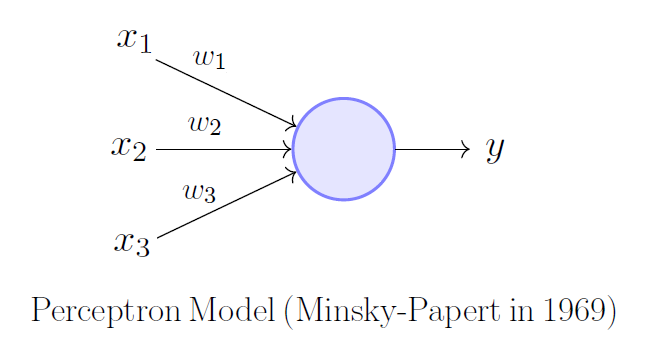
\includegraphics[width=8cm]{percep.png}}
\caption{\text{Perceptron Model}}
\end{center}
\end{figure}

\section{Definition}
The perceptron is an algorithm for supervised learning of binary classifiers. the perceptron is an algorithm for learning a binary classifier called a threshold function: a function that maps its input $\mathbf {x}$  (a real-valued vector) to an output value $ f(\mathbf {x} )$ (a single binary value):
$f(\mathbf{x})=\left\{\begin{array}{ll}{1} & {\text { if } \mathbf{w} \cdot \mathbf{x}+b>0} \\ {0} & {\text { otherwise }}\end{array}\right.$\\
where $ \mathbf {w}$  is a vector of real-valued weights,$ {\displaystyle \mathbf {w} \cdot \mathbf {x} }$ is the dot product$ {\displaystyle \sum _{i=1}^{m}w_{i}x_{i}} $where m is the number of inputs to the perceptron, and b is the bias. The bias shifts the decision boundary away from the origin and does not depend on any input value.\cite{DUMMY:1}
\par
It can be mathematically written as :
$$
\begin{aligned} \hat{y}=& \Theta\left(w_{1} x_{1}+w_{2} x_{2}+\ldots+w_{n} x_{n}+b\right) \\=& \Theta(\mathbf{w} \cdot \mathbf{x}+b) \\ & \text { where } \Theta(v)=\left\{\begin{array}{ll}{1} & {\text { if } v \geqslant 0} \\ {0} & {\text { otherwise }}\end{array}\right. \end{aligned}
$$
which tells us that it is a basic linear equation.
\section{Limitations}
\par
The Perceptron ,even though is the building block of all Artificial Neural Network models, is a linear binary classifier and hence can only solve simple problems upon learning ,for example learning
\begin{enumerate}[label=(\Alph*)]
\item \textbf{OR Gate} The logical or gate has the output \textbf{1} for all inputs except when both are \textbf{0}.  
\begin{figure}[H]
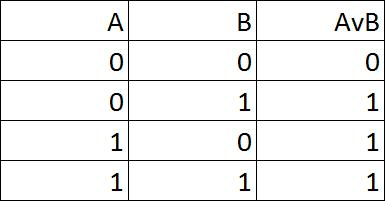
\includegraphics[width=8cm,height=7cm,center]{orgate.jpg}
\caption{\text{OR Gate}}
\end{figure}
When seen in a 2D plane with outputs plotted gives us the visual of OR gate in a graph. Now this graph can be seperated by a straight line as shown below to differentiate between the outputs with value 1 and value 0.\\
such a line's equation can be generated as $y$ with ,
$w 1=1, w 2=1, b=-0.5$ gives us the equation: $$y =A + B -0.5$$
\begin{figure}[H]
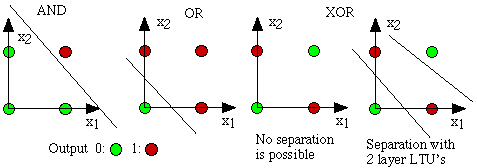
\includegraphics[center]{res.png}
\caption{\text{Perceptron Classification Result}}
\end{figure}
\item Simillary, All other basic logic gates can be made using a single perceptron. Whereas making a XOR Gate is impossible with just a single perceptron. To do this we require a network of these perceptron as we already know XOR can be represented as combination of AND \& OR gate in boolen equation as:
$$
\mathbf{A} \oplus \mathbf{B}=\mathbf{A} \overline{\mathbf{B}}+\overline{\mathbf{A}} \mathbf{B}
$$
\end{enumerate}

\chapter{\fontsize{16}{14}\textbf{Artificial Neural Networks\hfill}}
\section{Introduction}
\par
“Neural“ is an adjective for neuron, and “network” denotes a graph like structure.
Artificial Neural Networks are also referred to as “neural nets” , “artificial neural systems”, “parallel distributed processing systems”, “connectionist systems”.
Artificial Neural Network (ANNs) are programs designed to solve any problem by trying to mimic the structure and the function of our nervous system.
Neural networks are based on simulated neurons, Which are joined together in a variety of ways to form networks.
\begin{figure}[H]
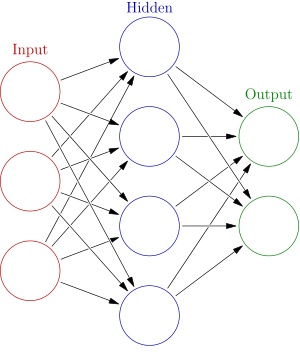
\includegraphics[height=7cm,center]{neural.png}
\caption{\text{Neural Network}}
\end{figure}
\newpage
\section{History}
Neural network simulations appear to be a recent development. However, this field was
established before the advent of computers, and has survived at least one major setback and
several eras. 
\par
Many importand advances have been boosted by the use of inexpensive computer emulations.
Following an initial period of enthusiasm, the field survived a period of frustration and disrepute.
During this period when funding and professional support was minimal, important advances
were made by relatively few reserchers. These pioneers were able to develop convincing
technology which surpassed the limitations identified by Minsky and Papert. Minsky and Papert,
published a book (in 1969) in which they summed up a general feeling of frustration (against
neural networks) among researchers, and was thus accepted by most without further analysis.
Currently, the neural network field enjoys a resurgence of interest and a corresponding increase
in funding. 
\par
The first artificial neuron was produced in 1943 by the neurophysiologist Warren McCulloch and
the logician Walter Pits. But the technology available at that time did not allow them to do too
much

\section{Architecture of neural networks}
\subsection{Feed-forward networks}
Feed-forward ANNs allow signals to travel one way only; from input to output. There
is no feedback (loops) i.e. the output of any layer does not affect that same layer. Feed-forward
ANNs tend to be straight forward networks that associate inputs with outputs. They are
extensively used in pattern recognition. This type of organisation is also referred to as bottom-up
or top-down. 
\begin{figure}[H]
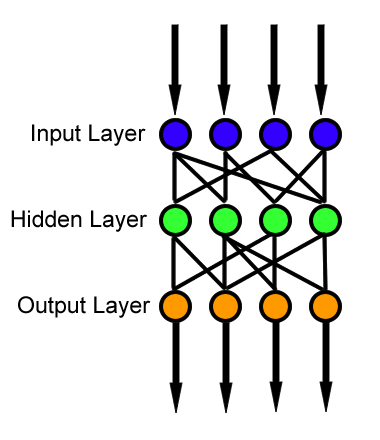
\includegraphics[height=7cm,center]{ffnn.png}
\caption{\text{Feed Forward Neural Network}}
\end{figure}
\subsection{Feedback networks}
Feedback networks can have signals travelling in both directions by introducing loops
in the network. Feedback networks are very powerful and can get extremely complicated.
Feedback networks are dynamic; their 'state' is changing continuously until they reach an
equilibrium point. They remain at the equilibrium point until the input changes and a new
equilibrium needs to be found. Feedback architectures are also referred to as interactive or
recurrent, although the latter term is often used to denote feedback connections in single-layer
organisations.

\begin{figure}[H]
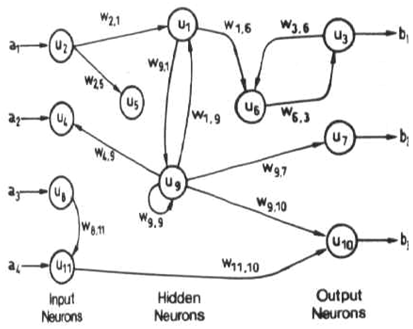
\includegraphics[height=5cm,center]{fbnn.png}
\caption{\text{Feed back Neural Network}}
\end{figure}
\newpage
\subsection{Network layers}
\par
The commonest type of artificial neural network consists of three groups, or layers, of units: a
layer of "input" units is connected to a layer of "hidden" units, which is connected to a layer of
"output" units.
\par
This simple type of network is interesting because the hidden units are free to construct their own
representations of the input. The weights between the input and hidden units determine when
each hidden unit is active, and so by modifying these weights, a hidden unit can choose what it
represents.
\begin{figure}[H]
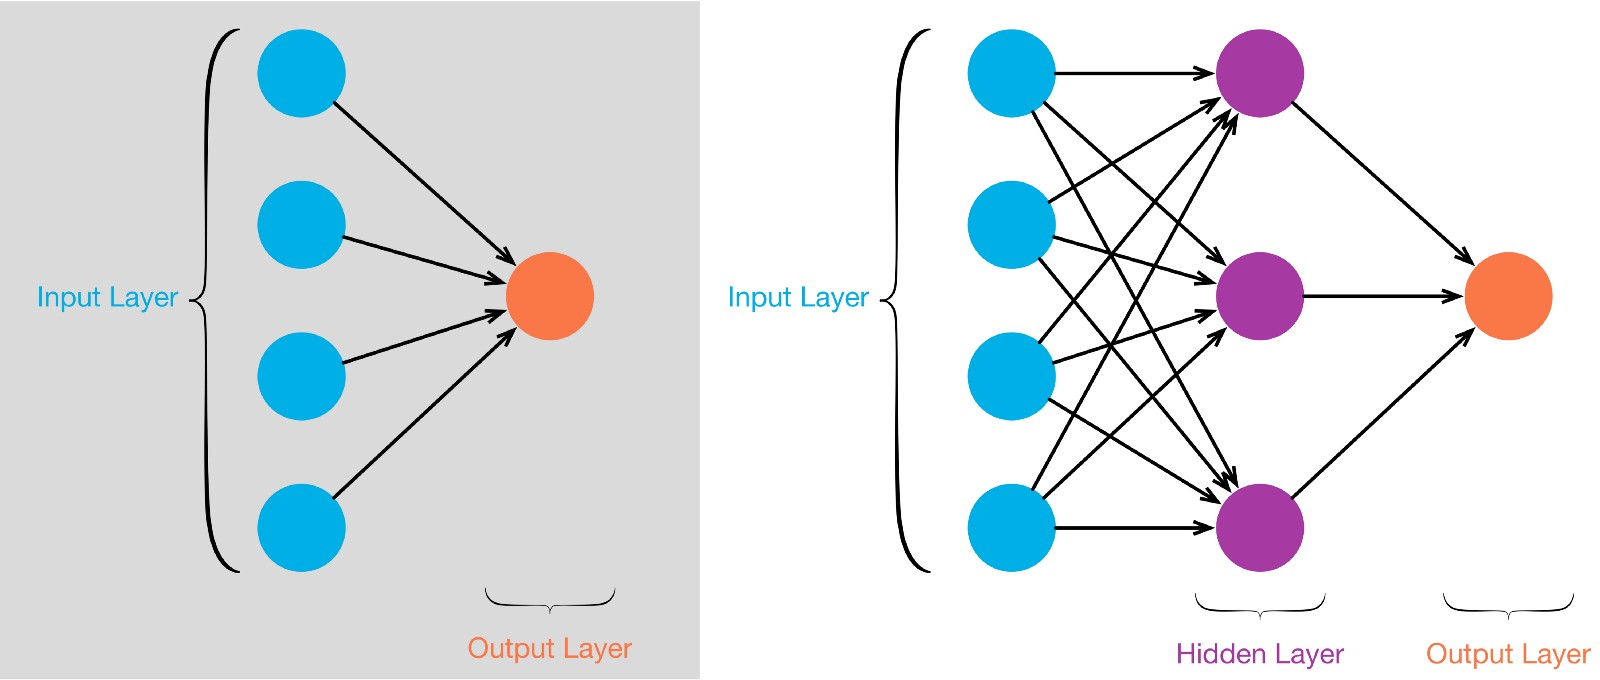
\includegraphics[width=15cm,height=7cm,center]{slvsml.jpeg}
\caption{\text{Single Layer VS Multi-layer Neural Network}}
\end{figure}
\par
We also distinguish single-layer and multi-layer architectures. The single-layer organisation, in
which all units are connected to one another, constitutes the most general case and is of more
potential computational power than hierarchically structured multi-layer organisations. In multilayer networks, units are often numbered by layer, instead of following a global numbering.

\newpage
\section{The Learning Process}
The memorisation of patterns and the subsequent response of the network can be categorised into
two general paradigms:
\begin{itemize}
\item \textbf{Associative mapping} in which the network learns to produce a particular pattern on the set of
input units whenever another particular pattern is applied on the set of input units. The associtive
mapping can generally be broken down into two mechanisms: 
\begin{itemize}
\item \textbf{Auto-association}: an input pattern is associated with itself and the states of input and output
units coincide. This is used to provide pattern completition, ie to produce a pattern whenever a
portion of it or a distorted pattern is presented. In the second case, the network actually stores
pairs of patterns building an association between two sets of patterns. 
\item \textbf{Hetero-association}: is related to two recall mechanisms:
\begin{itemize}
\item \textbf{Nearest-neighbour recall} where the output pattern produced corresponds to the input pattern
stored, which is closest to the pattern presented, and 
\item \textbf{Interpolative recall} where the output pattern is a similarity dependent interpolation of the
patterns stored corresponding to the pattern presented. Yet another paradigm, which is a variant
associative mapping is classification, ie when there is a fixed set of categories into which the
input patterns are to be classified. 
\end{itemize}
\end{itemize}
\item \textbf{Regularity detection} in which units learn to respond to particular properties of the input
patterns. Whereas in asssociative mapping the network stores the relationships among patterns,
in regularity detection the response of each unit has a particular 'meaning'. This type of learning
mechanism is essential for feature discovery and knowledge representation. 
\end{itemize}
Every neural network posseses knowledge which is contained in the values of the connections
weights. Modifying the knowledge stored in the network as a function of experience implies a
learning rule for changing the values of the weights.
\newpage
\chapter{\fontsize{16}{14}\textbf{CONCLUSION}}

\par
In the context of the reference taken from the research paper the ANN brings out the best result. This study illustrates how
this concept can be used to predict electricity energy
consumption in Hong Kong. When comparing accuracy in
predicting electricity energy consumption, it is found that
the decision tree model and neural network model perform
slightly better than other models in the summer and winter
phases, respectively. 
\par
Following are the advantages of ANN: 
\begin{itemize}
\item  Easy to use and understand. 
\item Can handle both categorical and numerical data. 
\item Resistant to outliers, hence require little data preprocessing. 
\item New features can be easily added. 
\item Can be used to build larger classifiers by using ensemble methods.
\end{itemize}

Following are the disadvantages of decision trees: - Prone to overfitting. - Require some kind of measurement as to how well they are doing. - Need to be careful with parameter tuning. - Can create biased learned trees if some classes dominate.
\par
In my opinion preventing the tree from growing too deep by stopping it before it perfectly classifies the training data. 

\newpage
\clearpage
\renewcommand{\bibname}{REFERENCES}
\bibliography{ref1} 
\bibliographystyle{ieeetr}
\begin{itemize}
\item[[2]]Yan YY. Climate and residential electricity consumption in Hong
Kong. Energy 1998;23:17–20. 
\item[[3]]Ranjan M, Jain VK. Modelling of electrical energy consumption in
Delhi. Energy 1999;24:351–61. 
\item[[4]]  Muller W, Wiederhold E. Applying decision tree methodology for
rules extraction under cognitive constraints. Eur J Oper Res
\item[[5]]Comparative study among different neural net learning
algorithms applied to rainfall time series.METEOROLOGICAL APPLICATIONS
Meteorol. Appl. 15: 273–280 (2008)
\item[[6]]HEART DISEASE PREDICTION USING DATA MINING TECHNIQUES.ICTACT JOURNAL ON SOFT COMPUTING, OCTOBER 2018
2002;136:282–9. 
\end{itemize}
\end{normalsize}
\end{document}